\section{Voting Protocol}

The section describes in details Voting and Tally stages. We assume that after the Preparation stage the following four sets are defined:
\begin{itemize}[leftmargin=5em, itemsep=0em]
    \item \textbf{Proposals} $\mathcal{P}:=\{p_1,\ldots, p_k \}$.
    \item \textbf{Voting committee} $\mathcal{C}:=\{c_1,\ldots, c_l \}$.
    \item \textbf{Voters} $\mathcal{V}:=\{v_1,\ldots, v_n \}$.
    \item \textbf{Experts} $\mathcal{E}:=\{e_1,\ldots, e_m \}$.
\end{itemize}

\subsection{Preliminaries}

\subsubsection{Basic Math}
The implementation\footnote{Implementation of all basic crypto can be found here:\\ \href{https://github.com/input-output-hk/treasury-crypto/tree/master/src/main/scala/io/iohk/core/crypto}{https://github.com/input-output-hk/treasury-crypto/../core/crypto}} of our scheme is based on elliptic curve groups for efficiency.
Let $\sigma:=(p,a,b,g,q,\zeta)$ be the elliptic curve domain parameters over $\FF_p$, consisting of a prime $p$ specifying the finite field $\FF_p$, two elements $a,b\in\FF_p$ specifying an elliptic curve $E(\FF_p)$ defined by
$E: y^2\equiv x^3 + ax + b \pmod p$,
a base point $g=(x_g,y_g)$ on $E(\FF_p)$, a prime $q$ which is the order of $g$, and an integer $\zeta$ which is the cofactor $\zeta=\#E(\FF_p)/q$.
We denote the cyclic group generated by $g$ by $\group$, and it is assumed that the DDH assumption holds over $\group$, that is for all p.p.t. adversary $\AAA$:
$$
\Adv(\AAA) = \left| \Pr\left[\begin{array}{l}x,y\leftarrow \ZZ_q; b\leftarrow\set{0,1};h_0=g^{xy};\\
h_1\leftarrow\group:\AAA(g,g^x,g^y,h_b)=b\\ 
\end{array}   \right]-\frac{1}{2} \right| \leq \epsilon(\lambda)
\enspace,$$
where $\epsilon(\cdot)$ is a negligible function.


\subsubsection{ElGamal Encryption} \label{sec:elgamal}
We employ lifted ElGamal encryption scheme as the candidate of the additively homomorphic public key cryptosystem in our protocol construction. It consists of the following p.p.t. algorithms:
\begin{itemize}
\item $\Gen(1^\lambda)$: take input as security parameter $\lambda$, and output $\sigma:=(p,a,b,g,q,\zeta)$.
\item $\Genpkc(\sigma)$: pick $\sk\leftarrow \ZZ_q^*$ and set $\pk:=h=g^{sk}$, and output $(\pk,\sk)$. 
\item $\Enc'_{\pk}(n;r)$: output $e:=(e_1,e_2)=(g^r,n\cdot h^r)$ is a regular ElGamal encryption, where $n\in E(\FF_p)$ is an EC point.
\item $\Dec'_{\sk}(e)$: output $n=e_2\cdot e_1^{-\sk}$ is a regular ElGamal decryption.
\item $\Enc_{\pk}(m;r)$: output $e:=(e_1,e_2)=(g^r,g^m h^r)$ is a lifted ElGamal encryption, where $m\in \ZZ_q^*$ is an integer.
\item $\Dec_{\sk}(e)$: output $m=\DL(\Dec'_{sk}(e))$, where $\DL(x)$ is a discrete logarithm of $x$. (Note that since $\DL(\cdot)$ is not efficient, the message space should be a small set, say $m\in \set{0,1}^\xi$, for $\xi\leq30$.)
\end{itemize}

It is well known that lifted ElGamal encryption scheme is IND-CPA secure under the DDH assumption. It has additively homomorphic property: $$\Enc_{\pk}(m_1;r_1) \cdot \Enc_{\pk}(m_2;r_2) = \Enc_{\pk}(m_1 + m_2 ;r_1+ r_2 )\enspace.$$

Remark: The key generation and decryption algorithm of the lifted ElGamal encryption can be efficiently distributed.

\subsubsection{Hybrid Encryption}
We employ a hybrid symmetric/assymetric encryption scheme for long messages that can not be encrypted directly with ElGamal  scheme. The basic idea is that a message is encrypted with a block cipher with a randomly generated symmetric key, whereas the key is encrypted with ElGamal and sent along the encrypted message. The hybrid encryption consists of the following algorithms:
\begin{itemize}
	\item $\Genpkc(\sigma)$: pick $\sk\leftarrow \ZZ_q^*$ and set $\pk:=h=g^{sk}$, and output $(\pk,\sk)$. 
	\item $\Genpkc^S(\sigma)$: pick $s\leftarrow \ZZ_q^*$ and set $\ck:=g^{s}$, and output $\ck$. 
	\item $\SEnc_{\ck}(m)$: output $e:=AESEnc_{H(ck)}(m)$, where $H$ is a cryptographic hash function and $AESEnc$ is an encryption method of AES block cipher.
	\item $\SDec_{\ck}(e)$: output $m:=AESDec_{H(ck)}(e)$, where $AESDec$ is a decryption method of AES block cipher.
	\item $\HEnc_{\pk}(m,r,ck)$: output $e:=(e_1,e_2)=(Enc'_{\pk}(ck,r), SEnc_{\ck}(m))$ is a hybrid encryption.
	\item $\HDec_{\sk}(e)$: output $m:=SDec_{\ck}(e_2))$, where $ck=Dec'_{\sk}(e_1)$.
\end{itemize}

\subsubsection{Pedersen Commitment}
In the unit vector zero-knowledge proof, we use Pedersen commitment as a building block. It is perfectly hiding and computationally binding under the discrete logarithm assumption. 
More specifically, it consists of the following $4$ PPT algorithms. Note that those algorithms (implicitly) take as input the same group parameters, $\param\leftarrow \Gen(1^{\lambda})$. 

\begin{itemize}
\item $\Gencom(\param)$: pick $s\leftarrow \ZZ_q^*$ and set $\ck:=h=g^{s}$, and output $\ck$. 
\item $\Com_{\ck}(m;r)$: output $c:=g^m h^r$ and $d:=(m,r)$.
\item $\Open(c, d)$: output $d:=(m,r)$. 
\item $\Verify_\ck(c,d)$: return $\valid$ if and only if  $c = g^m h^r$.
\end{itemize}

Pedersen commitment is also additively homomorphic, i.e.
$$
\Com_{\ck}(m_1;r_1)\cdot \Com_{\ck}(m_2;r_2) = \Com_{\ck}(m_1+m_2; r_1+r_2)\enspace.
$$

\subsection{Distributed Key Generation}
Distributed key generation (DKG) is a fundamental building block of the voting process in our proposed treasury system. Ideally, the protocol termination should be guaranteed when up to $t=\ceil{\frac{n}{2}} -1$ out of $n$ committee members are corrupted.  A naive way of achieving threshold distributed key generation is as follows. Each of the voting committee members $\VC_i$ first generates a public/private key pair $(\pk_i,\sk_i)\leftarrow\Genpkc(\param)$. Each $\VC_i$ then posts $\pk_i$ to the blockchain and use $(t+1,n)$-threshold \emph{verifiable secret sharing} (VSS) to share $\sk_i$ to all the other committee members. The combined voting public key can then be defined as $\pk:= \prod_{i=1}^{n} \pk_{i}$.

However, this approach is problematic in the sense that the adversary can influence the distribution of the final voting public key by letting the corrupted committee members abort selectively. Alternatively, we will adopt the distributed key generation protocol proposed by Gennaro {\em et al.}~\cite{GennaroDKG}. 
In a nutshell, the protocol lets the committee members $\VC_i$ first post a ``commitment'' of $\pk_i$. After sharing the corresponding $\sk_i$ via $(t+1,n)$-threshold VSS, the committee members $\VC_i$ then reveal $\pk_i$.
%
We will use the blockchain to realize the broadcast channel and peer-to-peer channels. We give a full description of our distributed key generation protocol.  It is adapted from the DKG proposed by Gennaro {\em et al.}, which allows us to accommodate up to $t < n/2$ malicious players in the protocol. That is, guaranteeing that with $ \floor{\frac{n}{2}}+1$ honest players, all the players should be able to agree on a uniformly random  public key $\pk$ such that no malicious players can influence the distribution of the generated public key. The corresponding secret key is shared among all the players.

\medskip
\noindent\textbf{Protocol description.}
Given $(g,h)$ as the common reference string (CRS), let $\VC:=\{\VC_1, \VC_2,...,\VC_k\}$ be the set of election committee members, and let $(\pk_{i},\sk_{i}),(\pk^*_{i},\sk^*_{i})$ be two pairs of public/secret keys\footnote{Note that we named public keys as \textit{pubKey} and \textit{committeePubKey} correspondingly in the definition of a committee registration transaction [\ref{ref:reg_tx}]} associated with $C_i, i \in [k]$. Note that $(\pk^*_{i},\sk^*_{i})$ is used to communicate with other committee members, while $(\pk_{i},\pk_{i})$ is used to generate a shared election key. The adversary is able to corrupt up to $t < k/2 $ committee members.\\

In the first round, each committee member $C_i$ sets $a_{i,0}=\sk_{i}$ and picks random $a_{i,1},...a_{i,t} $ and random $ a'_{i,0},...,a'_{i,t}$ where $t$ is the maximum number of members that can be corrupted. Each member then define two polynomials of degree t of the form:
\[ f_i(x) = a_{i,0}+a_{i,1}x+...+a_{i,t}x^t \]
\[ f'_i(x) = a'_{i,0}+a'_{i,1}x+...+a'_{i,t}x^t \]
Therefore, each committee member $\VC_i$ contributes $\sk_{i} = a_{i,0} = f(0)$ to the combined election secret key $\sk$.
Furthermore, to confirm the correctness of commitments, each member $\VC_i$ posts a corresponding commitment $E_{i,l} = g^{a_{i,l}}h^{a'_{i,l}}$, $l \in [0,t]$, on the blockchain. For every other member of the election committee, each $\VC_i$ computes $s_{i,j} = f_i(j) $ and $s'_{i,j} = f'_{i}(j) $ and posts to the blockchain, the encryption of $s_{i,j}$ and $ s'_{i,j}$ under the public key $\pk^*_{j}$ of $\VC_j$ (note: $j \neq i$). Note that only $\VC_j$ can decrypt these commitments. This signifies the end of the first round.\\

In the second round, each committee member $\VC_j$ fetches all $e_{i,j}$ and $e'_{i,j}$ encrypted under their public key from the blockchain and decrypt them using their private key $\sk^*_{j}$ to obtain their corresponding shares $s_{i,j}$ and $ s'_{i,j}$. In order to verify that the shares they have received are valid, each committee member checks if: $g^{s_{i,j}}h^{s'_{i,j}} = \prod_{l=0}^{t}(E_{i,l})^{i^l}$ for $i \in [k], i \neq j$.  Where this check fails, $\VC_j$ posts a complain against $\VC_i$ by revealing the decrypted shares and the evidence (in a form of a non-interactive ZK proof), that shares are decrypted correctly (see Fig.~\ref{fig:DKG} for more details).
Members with at least one valid complain against them are disqualified from participating in the key generation process.\\

In the third round, following the disqualification of some members, each qualified committee member $C_i,~i\in\JJJ$ posts $A_{i,l} := g^{a_{i,l}}$ for $ \ell \in [0,..,t] $ to the blockchain. Note that secret keys $sk_{i}$ of qualified committee members can be reconstructed as follows: $\sk_{i} := \sum_{j\in[\JJJ]} \gamma_{i} \cdot s_{i,j}$, where $\gamma_{i}:= \prod_{\ell\in \JJJ\setminus \{i\} } \frac{\ell}{\ell-i}$.\\

In the fourth round, each qualified committee member $C_i$ checks  if : $g^{s_{j,i}}= \prod_{\ell=0}^{t} (A_{j,\ell})^{i^\ell}$ for $j\in\JJJ, j\neq i$. Where the check fails, $\VC_i$ posts a complaint against $\VC_j$ together with the evidence $(s_{j,i},s'_{j,i})$ on the blockchain, such that $g^{s_{j,i}}h^{s'_{j,i}}= \prod_{\ell=0}^{t} (E_{j,\ell})^{i^\ell}$ and $g^{s_{j,i}}\neq  \prod_{\ell=0}^{t} (A_{j,\ell})^{i^\ell}$. Members with at least one valid complain against them are disqualified from further participation. \\

In the fifth and final round, each qualified committee member $\VC_i$ checks if complaints raised against other committee members in the fourth round are valid. For all members, against whom valid complaints in the forth round were raised, other qualified committee members post shares $s_{j,i}$ they received from them. Therefore, allowing everyone to reconstruct secret keys of failed committee members as: $\sk_{j} := \sum_{i\in[\JJJ]} \gamma_{j} \cdot s_{j,i}$, where $\gamma_{j}:= \prod_{\ell\in \JJJ\setminus \{j\} } \frac{\ell}{\ell-j}$, and redefine $A_{j,0}:= g^{\sk_{j}}$. 

Finally, the shared election public key is calculated as $\pk := \prod_{j\in[\JJJ]}  A_{j,0}$. Note that since all needed data to calculate $\pk$ is posted on the blockchain, every node in the network can reconstruct $\pk$ locally.\\

Note that, when implemented in a decentralized blockchain setting, it is supposed that all communications among committee members are done through the blockchain. It means that on each round they will post a transaction with relevant data that will also be checked by the whole network (where possible). At the end of the final round, every node in the network will be able to reconstruct a shared election public key without any additional messages from the committee. 

The full DKG protocol is summarized in Figure~\ref{fig:DKG}.\footnote{See implementation here:\\ \href{https://github.com/input-output-hk/treasury-crypto/tree/master/src/main/scala/io/iohk/protocol/keygen}{https://github.com/input-output-hk/treasury-crypto/.../protocol/keygen}} The NIZK used in Round 2 is described in Fig.~\ref{fig:ElgamalDecrNIZK}.\footnote{See implementation here:\\ \href{https://github.com/input-output-hk/treasury-crypto/blob/master/src/main/scala/io/iohk/protocol/nizk/ElgamalDecrNIZK.scala}{https://github.com/input-output-hk/treasury-crypto/../protocol/nizk/ElgamalDecrNIZK.scala}}

\FloatBarrier
% \end{boxfig}
\mybox{Distributed key generation $\Pi_{\textsc{DKG}}$}{white!40}{white!10}{
\footnotesize
\textbf{Round 1:}
Each committee member $C_i$ does the following:
\begin{itemize}
\item Set $a_{i,0}=sk_{i}$
\item Pick random $a_{i,1},a_{i,2},\ldots,a_{i,t},b_{i,0},b_{i,1},\ldots,b_{i,t} \leftarrow \ZZ_p$.
\item Define two polynomials $f_i(x):=\sum_{\ell=0}^{t} a_{i,\ell} x^\ell$ and $f'_i(x):=\sum_{\ell=0}^{t} b_{i,\ell} x^\ell$.
\item For $\ell\in[t]$, post $E_{i,\ell}: = g^{a_{i,\ell}} h^{b_{i,\ell}}$ on the blockchain.
\item For every other $C_j$, $j\in[k], j\neq i$, compute $s_{i,j}:= f_i(j)$ and $s'_{i,j}:= f'_i(j)$ and post $e_{i,j}\leftarrow \HEnc_{\pk^*_j}(s_{i,j}, r, ck_{i,j})$ and $e'_{i,j}\leftarrow \HEnc_{\pk^*_j}(s'_{i,j}, r', ck'_{i,j})$ on the blockchain, where $r,r'\leftarrow \ZZ_p$, $ck_{i,j},ck'_{i,j} \leftarrow E(\FF_p)$ are randomly generated. Only $C_j$ can decrypt these shares.
\end{itemize}

\textbf{Round 2:}
Each committee member $C_i$ does the following:
\begin{itemize}
\item Fetch $\{(e_{j,i}, e'_{j,i})\}_{j\in[k], j\neq i}$ from the blockchain, parse as $e_{j,i}=(e_{(j,i),1},e_{(j,i),2})$, $e'_{j,i}=(e'_{(j,i),1},e'_{(j,i),2})$, and use $\pk^*_i$ to decrypt them, obtaining the corresponding shares $\{(s_{j,i}, s'_{j,i})\}_{j\in[k], j\neq i}$.
\item For $j\in[k], j\neq i$, check if $g^{s_{j,i}}h^{s'_{j,i}}= \prod_{\ell=0}^{t} (E_{j,\ell})^{i^\ell}$. If not, post a complaint against $C_j$ by revealing the evidence: $(s_{j,i},s'_{j,i}, e_{j,i}, e'_{j,i},ck_{j,i},ck'_{j,i},\pi,\pi')$, where $\pi,\pi'$ are zero-knowledge proofs generated as follows (see Fig.~\ref{fig:ElgamalDecrNIZK} for full NIZK description):
\begin{equation*}
\pi \leftarrow\nizk\left\{\begin{array}{l} (e_{(j,i),1},\ck_{j,i}, \pk^*_i),(\sk^*_i): \\
 ck_{j,i}=\Dec'_{\sk^*_i}(e_{(j,i),1}) \wedge \pk^*_i=g^{\sk^*_i} \wedge (\pk^*_i,\sk^*_i)\in\RRR_{\textsc{PKE}} \end{array}\right\}
\end{equation*}
\item (One valid complain against $C_j$, $j\in[k]$ will disqualify $C_j$.)
\end{itemize}

\textbf{Round 3:} Define the indices of the qualified set of committee members as $\JJJ$. Each committee member $C_i$ does the following:
\begin{itemize}
\item For $\ell\in[t]$, post $A_{i,\ell} : = g^{a_{i,\ell}}$ to the blockchain.
\item Note that a secret key $sk_{i}$ of $C_i,~i\in\JJJ,$ can be reconstructed as follows: $\sk_{i} := \sum_{j\in[\JJJ]} \gamma_{i} \cdot s_{i,j}$, where $\gamma_{i}:= \prod_{\ell\in \JJJ\setminus \{i\} } \frac{\ell}{\ell-i}$.
\end{itemize}

\textbf{Round 4:} Each committee member $C_i$ does the following:
\begin{itemize}

\item For $j\in\JJJ, j\neq i$, check if $g^{s_{j,i}}= \prod_{\ell=0}^{t} (A_{j,\ell})^{i^\ell}$. If not, post a complaint against $C_j$ together with the evidence $(s_{j,i},s'_{j,i})$ on the blockchain, such that $g^{s_{j,i}}h^{s'_{j,i}}= \prod_{\ell=0}^{t} (E_{j,\ell})^{i^\ell}$ and $g^{s_{j,i}}\neq  \prod_{\ell=0}^{t} (A_{j,\ell})^{i^\ell}$.
\end{itemize}

\textbf{Round 5:} Each committee member $C_i$ does the following:
\begin{itemize}
\item If there is a valid complain against $C_j$, $j\in\JJJ$, then post the share $s_{j,i}$ on the blockchain. 
 (Everyone can reconstruct $\sk_j := \sum_{i\in[\JJJ]} \gamma_{j} \cdot s_{j,i}$, where $\gamma_{j}:= \prod_{\ell\in \JJJ\setminus \{j\} } \frac{\ell}{\ell-j}$, and calculate $A_{j,0}:= g^{\sk_j}$.)

\item Return the election public key as $\pk := \prod_{j\in[\JJJ]}  A_{j,0}$.
\end{itemize}
	
%\end{boxfig}
}{Distributed key generation $\Pi_{\textsc{DKG}}$\label{fig:DKG}}

\begin{boxfig}{\label{fig:ElgamalDecrNIZK}Non-Interactive Zero Knowledge proof for correct ElGamal decryption}{}
\begin{center}
$\nizk\{(\pk, C, M ),(\sk): M = \Dec'_{\sk}(C) \, \wedge \, \pk = g^{\sk}\}$
\end{center}

\textbf{Statement:} Public key, $\pk:=h \in\group$,  ciphertext $C: =(C_1, C_2 )$, and the plaintext $M:=g^m \in\group$

\textbf{Witness:} $\sk\in\ZZ_p$

\medskip
\textbf{Prover:}
\begin{itemize}
\item Pick random $w \leftarrow  {\ZZ_p}$; 
\item Compute $D=(C_1)^{sk}$ , $A_1 := g^w$, and $A_2 := (C_1)^w $
\item Compute $e = \hash(C,D,A_1,A_2)$ and  $ z = \sk*e + w$
\item Return $\pi:=(A_1,A_2,z)$
\end{itemize}

\textbf{Verifier:}
\begin{itemize}
\item Compute $D=\frac{C_2}{M}$
\item Compute $e = \hash(C,D,A_1,A_2)$
\item Verify that:
    \begin{itemize}
    \item $g^z = h^e \cdot A_1$, and
    \item $(C_1)^{z} = D^e \cdot A_2$ 
    \end{itemize}
\end{itemize}
\end{boxfig}

\FloatBarrier
\subsection{Ballots Casting}

Let $m$ be the number of experts. Let $e^{(m)}_i \in \{0,1\}^{m}$ be a unit vector, where its $i$-th, $i \in [1,..,m]$, coordinate is $1$ and the rest coordinates are $0$. Similarly, let  $e^{(3)}_j \in \{0,1\}^{3}$ be a unit vector. Denote $( e^{(m)}_i , e^{(3)}_j )$ as the concatenation of $e^{(m)}_i $ and $e^{(3)}_j$.  We also abuse the notation to denote  $e^{(\ell)}_0$ as an $\ell$-vector containing all $0$'s.  

The expert's choice  is represented by one of the unit vectors $(e^{(3)}_1, e^{(3)}_2, e^{(3)}_3)$, where $e^{(3)}_1$ stands for `Abstain', $e^{(3)}_2$ stands for `Yes', and $e^{(3)}_3$ stands for `No'.

The voter's choice is represented by the concatenation of two  unit vectors $( e^{(m)}_i , e^{(3)}_j )$, where $e^{(m)}_i$, $i\in[0,m]$ stands for delegation choice and $e^{(3)}_i$, $i\in[0,2]$ stands for voting choice. If the voter wants to vote directly, he creates a unit vector $( e^{(m)}_0 , e^{(3)}_j ), j \in \{1,2,3\}$. Otherwise, if the voter wants to delegate his voting power to $\EXP_i$, he sets $(e^{(m)}_i,\ e^{(3)}_0 )$, where $i \in [1,m]$ is an index of a registered expert. 

Before publishing voter's/expert's choices on the blockchain they are encrypted. Let us denote a coordinate-wise encryption of $e^{(\ell)}_i$ as $\Enc_{\pk}(e^{(\ell)}_i )$, i.e. 
\[\Enc_{\pk}(e^{(\ell)}_i ) = \Enc_{\pk}(e^{(\ell)}_{i,1}), \ldots, \Enc_{\pk}(e^{(1)}_{i,\ell}),\]
where $e^{(\ell)}_i = (e^{(\ell)}_{i,1},\ldots, e^{(\ell)}_{i,\ell})$ and $\pk$ is a shared election public key generated during the DKG stage.

Since tally is calculated homomorphically by summing up encrypted unit vectors, it is crucial to verify that encryptions are formed correctly (i.e., that they indeed encrypt unit vectors). To do so, each voter/expert creates a special zero-knowledge proof for each published encrypted unit vector that proves it is correct. The corresponding ZK proof is described in section [\ref{sec:SHVZK}].
Note that a voter/expert publishes a separate unit vector for each submitted proposal.

The protocol for ballot casting is depicted in Figure~\ref{fig:vote}.\footnote{See implementation here:\\ \href{https://github.com/input-output-hk/treasury-crypto/blob/master/src/main/scala/io/iohk/protocol/voting/Voter.scala}{https://github.com/input-output-hk/treasury-crypto/../protocol/voting/Voter.scala}}

\begin{boxfig}{\label{fig:vote}Ballots casting}{}
\footnotesize
	\textbf{Preparation phase:}
	\begin{itemize}
	    \item Retrieve shared election public key $\pk$ generated with $\Pi_{\textsc{DKG}}$ as desceibed in Figure~\ref{fig:DKG}.
	\end{itemize}	
	
	\textbf{Ballots casting phase:}
	\begin{itemize}
		\item Upon issuing a voting ballot, an expert $\EXP_i$ does the following:
		\begin{itemize}
			\item For each submitted proposal $p_k \in \mathcal{P}$: 
			\begin{itemize}
			    \item create a unit vector $e^{(3)}_{k,\ell}$ according to his choice (e.g, $e^{(3)}_{k,1}$ for "Abstain", $e^{(3)}_{k,2}$ for "Yes", and $e^{(3)}_{k,3}$ for "No");
			    \item pick randomness $r_{k,1},r_{k,2},r_{k,3}\leftarrow \ZZ_p$ and compute $c_{k,t}\leftarrow \Enc_{\pk}(e^{(3)}_{k,t}; r_{k,t})$, $t\in[3]$;
			    \item produce a unit vector proof $\pi_k$ showing that $\{c_{k,t}\}_{t\in[3]}$ encrypts a unit vector\footnote{Due to complexity of the NIZK proof, we described it in a separate section [\ref{sec:SHVZK}]}.
			\end{itemize}
			  
			\item Send transaction with $(Ballot, (\EXP_i, \{\{c_{k,t}\}_{t\in[3]}, \pi_k\}_{k \in |\mathcal{P}|}))$ to the blockchain.
		\end{itemize}	
		
		\item Upon issuing a voting ballot, a voter $\Voter_i$ does the following:
		\begin{itemize}
			\item For each submitted proposal $p_k \in \mathcal{P}$: 
			\begin{itemize}
			    \item create a unit vector $e^{(m+3)}_{k,\ell}$ so that:
			    \begin{itemize}
			        \item if $\Voter_i$ wants to delegate, then $e^{(m+3)}_{k,\ell}:= (e^{(m)}_{k,i}, e^{(3)}_0)$, where $i \in [1,m]$ is an index of an expert;
			        \item otherwise, if $\Voter_i$ wants to vote directly, then $e^{(m+3)}_{k,\ell}:= (e^{(m)}_0, e^{(3)}_{k,i})$, where $i \in \{1,2,3\}$ depends on the choice (Abstain, Yes, or No correspondingly);
			    \end{itemize}

			    \item pick randomness $r_{k,1},\ldots, r_{k,m+3}\leftarrow \ZZ_q$ and compute $u_{k,t}\leftarrow \Enc_{\pk}(e^{(m+3)}_{k,t}; r_{k,t})$, $t\in[m+3]$;
			    \item produce a unit vector proof $\pi_k$ showing that $\{c_{k,t}\}_{t\in[m+3]}$ encrypts a unit vector.
			\end{itemize}
			  
			\item Send transaction with $(Ballot, (\Voter_i, \{\{c_{k,t}\}_{t\in[m+3]}, \pi_k\}_{k \in |\mathcal{P}|}))$ to the blockchain.
		\end{itemize}	
	\end{itemize}
\end{boxfig}

\FloatBarrier
\subsection{Unit Vector ZK Proof}\label{sec:SHVZK}
We denote a unit vector of length $n$ as $\vec{e}_i^{(n)} = (e_{i,0},\ldots, e_{i,n-1})$,  where its $i$-th coordinate is $1$ and the rest coordinates are $0$. Note that in this section we diverge from the previously established notation, where $\vec{e}_0^{(n)}$ was defined as a vector of zeroes, now we do not consider zero-vectors at all and the lower index signifies the position of the "1" bit in the vector, e.g., $\vec{e}_0^{(5)}=(10000), \vec{e}_4^{(5)}=(00001)$.

Conventionally, to show a vector of ElGamal ciphertexts element-wise encrypt a unit vector, Chaum-Pedersen proofs~\cite{CP92} are used to show each of the ciphertexts encrypts either $0$ or $1$ (via Sigma OR composition) and the product of all ciphertexts encrypts $1$\footnote{This approach is implemented in \href{https://github.com/input-output-hk/treasury-crypto/tree/master/src/main/scala/io/iohk/protocol/nizk/unitvectornizk}{https://github.com/input-output-hk/treasury-crypto/.../protocol/nizk/unitvectornizk}. But note that it is not used in the final protocol.}. Such kind of proof is used in many well-known voting schemes, e.g., Helios. However, the proof size is linear in the length of the unit vector, and thus the communication overhead is quite significant when the unit vector length becomes larger. 

In this section, we propose a novel special honest verifier ZK  (SHVZK)\footnote{See implementation here: \href{https://github.com/input-output-hk/treasury-crypto/tree/master/src/main/scala/io/iohk/protocol/nizk/shvzk}{https://github.com/input-output-hk/treasury-crypto/.../protocol/nizk/shvzk}} proof for a unit vector that allows a prover to convince a verifier that the vector of ciphertexts $(C_0,\ldots, C_{n-1})$ encrypts a unit vector $\vec{e}_i^{(n)}$, $i\in[0, n-1]$ with $O(\log n)$  proof size. Without loss of generality, assume $n$ is a perfect power of $2$. If not, we append $\Enc_{\pk}(0;0)$ (i.e., trivial ciphertexts) to make the total number of ciphertexts to be the next power of $2$. We transform the proposed SHVZK protocol to a non-interactive ZK (NIZK) using the Fiat-Shamir heuristic.

The basic idea of our construction is inspired by \cite{Groth2015}, where Groth and Kohlweiss proposed a Sigma protocol for the prover to show that he knows how to open one out of many commitments. The key idea behind our construction is that there exists a data-oblivious algorithm that can take input as $i \in [0,..,n-1]$ and output the unit vector $\vec{e}_i^{(n)}$. Let $i_1,\ldots, i_{\log n}$ be the binary representation of $i$. The algorithm is depicted in Fig.~\ref{fig:alg_unit}.

\myhalfbox{The algorithm that maps $i\in[0,n-1]$ to $\vec{e}_i^{(n)}$}{white!40}{white!10}{
\footnotesize
\textbf{Input:} index $i=(i_1,\ldots, i_{\log n})\in \{0,1\}^{\log n}$

\textbf{Output:} unit vector $\vec{e}_i^{(n)}= (e_{i,0},\ldots, e_{i,n-1}) \in \{0,1\}^n$ \\

1. For $\ell\in[\log n]$, set $b_{\ell,0} := 1- i_\ell$ and $b_{\ell,1} := i_\ell$;

2. For $j\in[0,n-1]$, set $e_{i,j}:= \prod_{\ell = 1}^{\log n} b_{\ell, j_\ell}$, where $j_1,\ldots, j_{\log n}$ is the binary representation of $j$;

3. Return $\vec{e}_i^{(n)}= (e_{i,0},\ldots, e_{i,n-1})$;	

}{The algorithm that maps $i\in[0,n-1]$ to $\vec{e}_i^{(n)}$\label{fig:alg_unit}}

 Intuitively, we let the prover first bit-wisely commit the binary presentation of $i\in[0,n-1]$ for the unit vector $\vec{e}_i^{(n)}$. The prover then shows that each of the commitments of $(i_1,\ldots, i_{\log n})$ indeed contain $0$ or $1$, using the Sigma protocol proposed in Section 2.3 of \cite{Groth2015}. Note that in the 3rd move of such a Sigma protocol, the prover reveals a degree-$1$ polynomial of the committed message.  Denote $z_{\ell,1}:=i_\ell x + \beta_\ell$, $\ell\in[\log n]$ as the corresponding degree-$1$ polynomials, where $\beta_\ell$ are chosen by the prover and $x$ is chosen by the verifier. By linearity, we can also define $z_{\ell,0}:= x - z_{\ell,1 }= (1-i_\ell) x -\beta_\ell$, $\ell\in[\log n]$.  According to the algorithm described in Fig.~\ref{fig:alg_unit}, for $j\in[0,n-1]$, let  $j_1,\ldots, j_{\log n}$ be the binary representation of $j$, and the product $\prod_{\ell=1}^{\log n} z_{\ell, j_\ell}$ can be viewed as a degree-$(\log n)$ polynomial of the form
$$
p_j(x) = e_{i,j} x^{\log n} + \sum_{k=0}^{\log n -1} p_{j,k} x^k 
$$
for some $p_{j,k}$, $k\in[0,\log n -1]$. We then use batch verification to show that each of $C_j$ indeed encrypts $e_{i,j}$. More specifically, for a randomly chosen $y\leftarrow \ZZ_p$, let $E_j:=(C_j )^{x^{\log n}} \cdot \Enc(-p_j(x);0)$; the prover needs to show that $E:= \prod_{j=0}^{n-1} (E_j) ^{y^j} \cdot \prod_{k=0}^{\log n -1} (D_k) ^{x^k}$ encrypts $0$, where $D_\ell:= \Enc_{\pk}(\sum_{j=0}^{n-1} (p_{j,\ell} \cdot y^j) ; R_{\ell})$, $\ell\in[0,\log n -1]$ with fresh randomness $R_\ell\in\ZZ_p$. The construction is depicted in Fig.~\ref{fig:unit_zk_prover}. Both the prover and the verifier shares a common reference string (CRS), which is a Pedersen commitment key that can be generated using random oracle. %Let $\Com_{\ck}(m;r)$ denote the Pedersen commitment of $m\in\ZZ_p$ using randomness $r\in_ZZ_p$ under key $\ck$.
The prover first commits to each bits of the binary representation of $i$, and the commitments are denoted as $I_\ell$, $\ell\in[\log n]$. Subsequently, it produces $B_\ell,A_\ell$ as the first move of the Sigma protocol in Sec.~2.3 of \cite{Groth2015} showing $I_\ell$ commits to $0$ or $1$. Jumping ahead, later the prover will receive a challenge $x\leftarrow \{0,1\}^\lambda$, and then it computes the third move of the Sigma protocols by producing $\{z_\ell,w_\ell,v_\ell\}_{\ell=1}^{\log n}$. To enable batch verification, before that, the prover is given another challenge $y\leftarrow \{0,1\}^\lambda$ in the second move. 

The verification consists of two parts (Fig.~\ref{fig:unit_zk_verifier}). In the first part, the verifier checks the following equations to ensure that $I_\ell$ commits to $0$ or $1$.
\begin{itemize}
\item $(I_\ell)^x \cdot B_\ell = \Com_{\ck}(z_\ell; w_\ell)$
\item $(I_\ell)^{x-z_\ell} \cdot A_\ell = \Com_{\ck}(0; v_\ell)$
\end{itemize}
In the second part, the verifier checks if
$$
\prod_{j=0}^{n-1} \big( (C_j )^{x^{\log n}} \cdot \Enc_{\pk}(-\prod_{\ell=1}^{\log n} z_{\ell, j_\ell};0)\big) ^{y^j} \cdot \prod_{\ell=0}^{\log n -1} (D_\ell)^{x^\ell}
$$
is encryption of $0$ by asking the prover to reveal the randomness.

\mybox{Unit vector ZK argument (Prover)}{white!40}{white!10}{
\footnotesize
\textbf{CRS:} the commitment key $\ck=hash(\pk)$

\textbf{Statement:} the public key $\pk$ and the ciphertexts $C_0:=  \Enc_{\pk}(e_{i,0};r_0),\ldots, C_{m-1}:=\Enc_{\pk}(e_{i,m-1};r_{m-1})$

\textbf{Witness:} the unit vector $\vec{e}_i^{(m)} \in \{0,1\}^m$ and the randomness $r_0,\ldots, r_{m-1} \in \ZZ_p$
\\~\\
\textbf{Prover:}
\begin{itemize}

\item If the number of ciphertexts $m$ is not a perfect power of 2, extend the set with $C_{j}:=\Enc_{\pk}(0;0), j \in [m,..,n-1]$, where $n$ is a perfect power of 2

\item Let $\{i_k\}_{k \in [0,..,log(n)-1]}$ be a binary representation of the index $i$ (e.g. if $i=3$ and $n=5$, its binary represantation is "00011", so that $i_0=0$, $i_1=0$, $i_2=0$, $i_3=1$, $i_4=1$)

\item For $\ell = 0,\ldots, \log n-1$ do the following:
    \begin{itemize}
    \item Pick random $\alpha_\ell,\beta_\ell,\gamma_\ell,\delta_\ell \leftarrow \ZZ_p$;
    \item Compute $I_\ell:=\Com_{\ck}(i_\ell; \alpha_\ell)$, $B_\ell:=\Com_{\ck}(\beta_\ell; \gamma_\ell)$ and $A_\ell:=\Com_{\ck}(i_\ell\cdot \beta_\ell; \delta_\ell)$;
    \end{itemize}

\item Compute first verifier challange (using Fiat-Shamir heuristic):
\[c_y=hash(\pk\ |\ \{C_l\}_{\ell=0}^{n-1}\ |\ \{I_\ell,B_\ell,A_\ell\}_{\ell=0}^{\log n-1})\]

\item For $j = 0,\ldots, n-1$ compute polynomials $p_j(x)$ of the following form:
\[p_j(x) = e_{i,j} x^{\log n} + \sum_{k=0}^{\log n -1} p_{j,k} x^k,\]
where $e_{i,j}$ is a $j$-th bit in the vector $\vec{e}_i^{(m)}$ and $p_{j,k}, k \in [0,..,log(n)-1]$ is a $k$-th coefficient of the polynomial $p_{j}$.\\
A polynomials $p_j(x)$ can be constructed using the following procedure:
\begin{itemize}
    \item Let $j_k, k \in [0,..,\log n-1]$ be a binary representation of the index $j$
    \item Compute $p_j(x)=\prod_{\ell=0}^{\log n-1} z_{\ell}^{j_\ell}$, where $j_\ell \in \{0,1\}$ and
    \[z^1_{\ell}=i_{\ell} x + \beta\]
    \[z^0_{\ell}=x-z^1_{\ell}=(1-i_{\ell}) x - \beta\]
\end{itemize}

\item For $\ell = 0,\ldots, \log n-1$ compute $D_{\ell}$ as follows:
    \begin{itemize}
    \item Pick random $R_\ell\leftarrow \ZZ_p$, and 
    \item Compute $D_\ell:=\Enc_{\pk}\big(\sum_{j=0}^{n-1} (p_{j,\ell} \cdot y^j);R_\ell \big)$
    \end{itemize}

\item Compute second verifier challange (using Fiat-Shamir heuristic):
\[c_x=hash(\pk\ |\ \{C_l\}_{\ell=0}^{n-1}\ |\ \{I_\ell,B_\ell,A_\ell\}_{\ell=0}^{\log n-1})\ |\ \{D_l\}_{\ell=0}^{\log n-1})\]

\item For $\ell = 0,\ldots, \log n-1$ compute $z_{\ell}, w_{\ell}$ and $v_{\ell}$ as follows:
    \begin{itemize}
        \item $z_\ell:= i_\ell \cdot c_x + \beta_\ell$
        \item $w_\ell:= \alpha_\ell \cdot c_x + \gamma_\ell$
        \item $v_\ell:= \alpha_\ell (c_x-z_\ell) + \delta_\ell$
    \end{itemize}

\item Compute $R:= \sum_{j=0}^{n-1}( r_j \cdot (c_x)^{\log n} \cdot (c_y)^j)  + \sum_{\ell=0}^{\log n -1} (R_\ell \cdot (c_x)^\ell)$

\item Return proof $\pi:=(\{I_\ell,B_\ell,A_\ell\}_{\ell=0}^{\log n-1}),\ \{D_l\}_{\ell=0}^{\log n-1}),\ \{z_\ell,w_\ell,v_\ell\}_{\ell=0}^{\log n-1},\ R)$
\end{itemize}
}{Unit vector ZK argument: proof creation  \label{fig:unit_zk_prover}}

\mybox{Unit vector ZK argument (Verifier)}{white!40}{white!10}{
\footnotesize
\textbf{CRS:} the commitment key $\ck=hash(\pk)$

\textbf{Statement:} the public key $\pk$ and the ciphertexts $C_0:=  \Enc_{\pk}(e_{i,0};r_0),\ldots, C_{m-1}:=\Enc_{\pk}(e_{i,m-1};r_{m-1})$

\textbf{Proof:} $\pi:=(\{I_\ell,B_\ell,A_\ell\}_{\ell=0}^{\log n-1}),\ \{D_l\}_{\ell=0}^{\log n-1}),\ \{z_\ell,w_\ell,v_\ell\}_{\ell=0}^{\log n-1},\ R)$
\\~\\
\textbf{Verification:}

\begin{itemize}
    \item If the number of ciphertexts $m$ is not a perfect power of 2, extend the set with $C_{j}:=\Enc_{\pk}(0;0), j \in [m,..,n-1]$, where $n$ is a perfect power of 2
    \item Compute first verifier challenge: $c_y=hash(\pk\ |\ \{C_l\}_{\ell=0}^{n-1}\ |\ \{I_\ell,B_\ell,A_\ell\}_{\ell=0}^{\log n-1})$
    \item Compute second verifier challenge: $c_x=hash(\pk\ |\ \{C_l\}_{\ell=0}^{n-1}\ |\ \{I_\ell,B_\ell,A_\ell\}_{\ell=0}^{\log n-1})\ |\ \{D_l\}_{\ell=0}^{\log n-1})$
    \item Verify that for $\ell = 0,\ldots, \log n-1$ the following equations are true:
        \begin{itemize}
        \item $(I_\ell)^{c_x} \cdot B_\ell = \Com_{\ck}(z_\ell; w_\ell)$
        \item $(I_\ell)^{c_x-z_\ell} \cdot A_\ell = \Com_{\ck}(0; v_\ell)$
        \end{itemize}
    \item Verify the following equation is true: 
    \[\prod_{j=0}^{n-1} \big((C_j)^{(c_x)^{\log n}} \cdot \Enc_{\pk}(-\prod_{\ell=0}^{\log n-1} z_{\ell}^{j_\ell};0)\big)^{(c_y)^j} \cdot \prod_{\ell=0}^{\log n -1} (D_\ell)^{(c_x)^\ell}= \Enc_{\pk}(0;R),\]
    where $z_{j}^{1} = z_j$, $z_{j}^{0} = c_x-z_j$, and $j_\ell \in \{0,1\}$ is a binary representation of $j$, $\ell \in [0,..,\log n-1]$.
\end{itemize}	
}{Unit vector ZK argument: proof verification  \label{fig:unit_zk_verifier}}

\FloatBarrier
\subsection{Tally Protocol}

At the tally stage, committee members jointly decrypt the results of the voting without revealing personal choices of experts and voters. 

Let denote as $\BBB^E:=\{B^E_1,\ldots, B^E_m \}$ a set of ballots received from experts and as $\BBB^V:=\{B^V_1,\ldots, B^V_n \}$ a set of ballots received from voters. Recall that a ballot contains encrypted unit vectors with choices (one unit vector for each proposal). Unit vectors of experts are $3$-bits long, while unit vectors of voters are $(m+3)$-bits long, where $m$ is the number of registered experts.

Without loss of generality, let assume that we have only one proposal, so that a ballot contains only one encrypted unit vector. Let denote bit-wise encryptions of a unit vector of a voter $V_i$ as $c_{v_i,j},\ j\in [0,..,m+2]$ and an encrypted unit vector of an expert $E_i$ as $c_{e_i,j},\ j\in [0,..2]$. Note that $c_{v_i,j},\ j\in [0,..,m-1]$ encrypt bits of a voter's unit vector that signify his delegation choice, while the rest of encrypted bits $c_{v_i,j},j\ \in [m,m+1,m+2]$ signify his voting choice ("Abstain","Yes","No").

Joint decryption is accomplished in two steps. At the first step, the number of delegations is calculated and jointly decrypted. To do so, the number of delegations for each expert is calculated homomorphically by summing up delegations part of voter's unit vectors (i.e., first $m$ bits). Then each committe member produces a decryption share with his secret key, that was used to generate shared election public key. Given decryption shares from all members, the number of delegations to each expert can be decrypted.

At the second step, the number of votes for each choice ("Abstain","Yes","No") is calculated homomorphically by summing up corresponding part of voter's and expert's unit vectors (weighed by the voting power for voters and delegated voting power for experts). Then, committe members produce decryption shares, which allows everyone to decrypt and verify the final tally.

The full protocol is described in Fig.~\ref{fig:tally1} and Fig.~\ref{fig:tally2}.\footnote{See implementation here:\\ \href{https://github.com/input-output-hk/treasury-crypto/blob/master/src/main/scala/io/iohk/protocol/voting/Tally.scala}{https://github.com/input-output-hk/treasury-crypto/../protocol/voting/Tally.scala}\\ \href{https://github.com/input-output-hk/treasury-crypto/blob/master/src/main/scala/io/iohk/protocol/decryption/DecryptionManager.scala}{https://github.com/input-output-hk/treasury-crypto/../protocol/decryption/DecryptionManager.scala}} Note that in case of several proposals, the protocol is performed for each proposal separately in parallel (for better efficiency, committee members may combine published data into a single transaction).

\begin{boxfig}{\label{fig:tally1}Tally (Rounds 1,2)}{}
\footnotesize
\textbf{Entities:}\\
    \hspace*{6mm} \textbf{Committee members} $\mathcal{C}:=\{C_1,\ldots, C_l \}$. Note that here we refer to the members that were qualified after the DKG stage.\\
    \hspace*{6mm} \textbf{Voters} $\mathcal{V}:=\{V_1,\ldots, V_n \}$.\\
    \hspace*{6mm} \textbf{Experts} $\mathcal{E}:=\{E_1,\ldots, E_m \}$\\

\textbf{Input data:}\\
    \hspace*{6mm} \textbf{Set of voter's ballots:} $C_V:=\{c_{v_1},\ldots, c_{v_n} \}$, where $c_{v_i}=\{c_{v_i,0},\ldots,c_{v_i,m+2}\}$ is an encrypted unit vector with choice of a voter $V_i$.\footnote{\label{note1}We consider only one proposal per ballot, so there is only one encrypted unit vector}\\
    \hspace*{6mm} \textbf{Set of expert's ballots:} $C_E:=\{c_{e_1},\ldots, c_{e_m} \}$, where $c_{e_i}=\{c_{e_i,0},c_{e_i,1},c_{e_i,2}\}$ is an encrypted unit vector with choice of an expert $E_i$.\\

\textbf{Round 1 (delegation decryption):}
Each committee member $C_j$ does the following:
\begin{itemize}
    \item For $i = 1,\ldots, m$ compute homomorphically the number of delegations $d_{e_i}$ for each expert $E_i$:
    \[d_{e_i}=\prod_{l=0}^{n-1} (c_{v_l,i})^{\alpha_l},\]
    where $\alpha_l$ is a voting power of the voter $V_l$ (amount of deposited stake). 
    \item For $i = 1,\ldots, m$ compute decryption shares for delegation sums as follows:
    \begin{itemize}
        \item Parse $d_{e_i}$ to $(d_{e_i,1}, d_{e_i,2})$ (recall that $c_{e_i}$ and, correspondingly, $d_{e_i}$ are ElGamal ciphertexts, which comprise of 2 group elements [\ref{sec:elgamal}])
        \item Compute $D_{j,e_i}=(d_{e_i,1})^{sk_j}$, where $sk_j$ is a secret key\footnote{Here we refer to the secret key $sk_j$ that was used to generate shared election public key and for which a corresponding $pk_j$ was registered by $C_j$.} of the committee member $C_j$, and a proof $\pi_i$ that the share is generated correctly (see Fig.~\ref{fig:DecrShareNIZK} for NIZK description):
        \begin{equation*}
        \pi_{j,i}\leftarrow\nizk\left\{\begin{array}{l} (\pk_j, d_{e_i,1}, D_{j,e_i}),(\sk_j): \\
         D_{j,e_i}=(d_{e_i,1})^{sk_j} \; \wedge pk_j=g^{sk_j} \; \wedge \;  (\pk_j,\sk_j)\in\RRR_{\textsc{PKE}} \end{array}\right\}
        \end{equation*}
    \end{itemize}
    \item Publish $\{D_{j,e_i}, \pi_i\}_{i \in [m]}$ to the blockchain
\end{itemize}

Committee members $C_j, j \in \FFF$, that failed to submit decryption shares are disqualified from further participation.
\\~\\
\textbf{Round 2 (delegation decryption shares recovery):}\\
Each qualified committee member $C_i,\ i \in \JJJ$ does the following:
\begin{itemize}
    \item If there are such committee members $C_j,\ j \in \FFF$, who failed to post valid decryption shares, then $C_i$ posts to the blockchain shares $s_{j,i},\ j \in \FFF$ of $C_j$'s secret key obtained during the Round 1 of the DKG protocol (Figure~\ref{fig:DKG}).
    \item Everyone can reconstruct a secret key\footnote{Note that there should be more than $l/2$ shares, where $l$ is the number of committee members, to be able to reconstruct the secret key} of $C_j$: $sk_j := \sum_{i\in[\JJJ]} \gamma_{j} \cdot s_{j,i}$, where $\gamma_{j}:= \prod_{\ell\in \JJJ\setminus \{j\} } \frac{\ell}{\ell-j}$,\\
    and reconstruct his decryption shares $D_{j,e_i}$.
\end{itemize}
\vspace*{2mm}
After obtaining all decryption shares $D_{j,e_i}$ from all committee members $C_j,\ j\in[1,..,l]$, everyone can decrypt delegation results as follows:
\begin{itemize}
    \item For $i = 1,\ldots, m$, where $m$ is the number of experts compute $D_{e_i}=\prod_{j=1}^{l} D_{j,e_i}$, where $l$ is the number of committee members.
    \item Compute number of delegations to each expert $E_i$ as $dlg_{i}=DLOG_g(\dfrac{d_{e_i,2}}{D_{e_i}})$, where $d_{e_i,2}$ is obtained during the Round 1 and $DLOG$ is a discrete logarithm for the resulting group element. Note that the logarithm is the number of delegations so it can be effectively found by brute force.\\
\end{itemize}
\textbf{Round 3 (tally results decryption):} see continuation on Fig.~\ref{fig:tally2}
\end{boxfig}

\begin{boxfig}{\label{fig:tally2}Tally (Rounds 3,4)}{}
\textbf{Round 3 (tally results decryption):}
Each qualified committee member $C_j,\ j\in\JJJ$ does the following:
\begin{itemize}
    \item For $i = 0,..,2$ compute homomorphically the tally result $r_i$ for each choice $i\in\{0,1,2\}$ ("Abstain","Yes","No" correspondingly) as follows:
    \[r_i^E=\prod_{j=1}^{m} (c_{e_j,m+i})^{dlg_j},\hspace*{3mm} r_i^V=\prod_{j=1}^{n} (c_{v_j,m+i})^{\alpha_j}\]
    \[r_i=r_i^E \cdot r_i^V\]
    where $dlg_j$ is a delegated voting power to the expert $E_j$ and $\alpha_j$ is a voting power of the voter $V_j$ (amount of deposited stake). 
    \item For $i = 0,.., 2$ compute decryption shares for tally results as follows:
    \begin{itemize}
        \item Parse $r_i$ to $(r_{i,1}, r_{i,2})$ (recall that $r_{i}$ is an ElGamal ciphertext, which comprises 2 group elements [\ref{sec:elgamal}])
        \item Compute decryption share $R_{j,i}=(r_{i,1})^{sk_j}$, where $sk_j$ is a secret key of the committee member $C_j$, and a proof $\pi_{j,i}$ that the share is generated correctly (see Fig.~\ref{fig:DecrShareNIZK} for NIZK description):
        \begin{equation*}
        \pi_{j,i}\leftarrow\nizk\left\{\begin{array}{l} (\pk_j, r_{i,1}, R_{j,i}),(\sk_j): \\
         R_{j,i}=(r_{i,1})^{sk_j} \; \wedge pk_j=g^{sk_j} \; \wedge \;  (\pk_j,\sk_j)\in\RRR_{\textsc{PKE}} \end{array}\right\}
        \end{equation*}
    \end{itemize}
    \item Publish $\{R_{j,i}, \pi_{j,i}\}_{i \in [0,..,2]}$ to the blockchain
\end{itemize}
Committee members $C_j, j \in \FFF'$, that failed to submit decryption shares are disqualified from further participation.
\\~\\
\textbf{Round 4 (tally decryption shares recovery):}

Each qualified committee member $C_i,\ i \in \JJJ'$ does the following:
\begin{itemize}
    \item If there are such committee members $C_j,\ j \in \FFF'$, who failed to post valid decryption shares, then $C_i$ posts to the blockchain shares $s_{j,i},\ j \in \FFF'$ of $C_j$'s secret key obtained during the Round 1 of the DKG protocol (Figure~\ref{fig:DKG}).
\end{itemize}

Everyone can reconstruct a secret key of $C_j,\ j\in\FFF'$: $sk_j := \sum_{i\in[\JJJ']} \gamma_{j} \cdot s_{j,i}$, where $\gamma_{j}:= \prod_{\ell\in \JJJ'\setminus \{j\} } \frac{\ell}{\ell-j}$\\\\
Everyone reconstructs missing decryption shares of disqualified committee members $C_j,\ j\in\FFF\cup\FFF'$ as $R_{j,i}=(r_{i,1})^{sk_j}$ for $i\in[0,..,2]$.\\\\
After obtaining all decryption shares $R_{j,i}$ from all committee members $C_j,\ j\in[1,..,l]$, everyone can decrypt tally results as follows:
\begin{itemize}
    \item For $i = 0,.., 2$ compute $R_i=\prod_{j=1}^{l} R_{j,i}$, where $l$ is the number of committee members.
    \item Compute number of votes for each choice $i\in\{0,1,2\}$ as $res_{i}=DLOG_g(\dfrac{r_{i,2}}{R_i})$, where $r_{i,2}$ is computed as in Round 3 and $DLOG$ is a discrete logarithm for the resulting group element. Note that the logarithm is the number of votes so it can be effectively found by brute force.\\
\end{itemize}
\end{boxfig}

\FloatBarrier
\begin{boxfig}{\label{fig:DecrShareNIZK}Non-Interactive Zero Knowledge proof for correct ElGamal decryption share (note that this NIZK is basically the same as ElGamal decryption NIZK in Fig.~\ref{fig:ElgamalDecrNIZK} except slightly different interface)}{}
\begin{center}
$\nizk\{(\pk, C, D ),(\sk): D = (C_1)^{\sk} \, \wedge \, \pk = g^{\sk}\}$
\end{center}

\textbf{Statement:} Public key, $\pk:=h \in\group$,  ciphertext $C: =(C_1, C_2 )$, and the decryption share $D:=(C_1)^{sk} \in\group$

\textbf{Witness:} $\sk\in\ZZ_p$

\medskip
\textbf{Prover:}
\begin{itemize}
\item Pick random $w \leftarrow  {\ZZ_p}$; 
\item Compute $A_1 := g^w$, and $A_2 := (C_1)^w $
\item Compute $e = \hash(C,D,A_1,A_2)$ and  $ z = \sk*e + w$
\item Return $\pi:=(A_1,A_2,z)$
\end{itemize}

\textbf{Verifier:}
\begin{itemize}
\item Compute $d$
\item Compute $e = \hash(C,D,A_1,A_2)$
\item Verify that:
    \begin{itemize}
    \item $g^z = h^e \cdot A_1$, and
    \item $(C_1)^{z} = D^e \cdot A_2$ 
    \end{itemize}
\end{itemize}
\end{boxfig}

\subsection{Distributed Randomness Generation}

As it was previously outlined in [\nameref{sec:overview}], randomness generation is done by committee members. It is split into two phases:
\begin{enumerate}
	\item \textbf{Random value commitment}, and
	\item \textbf{Randomness revealing}.
\end{enumerate}

Commitment phase is done during the post-voting stage. At this phase each qualified\footnote{By qualified we mean a committee member that has not been disqualified during any of the previous stages (DKG, Tally)} committe member generates a random value and submits its encryption (under his private key) to the blockchain. No one else knows the committed random values of committee members. The commitment phase is formilized at Fig.~\ref{fig:rand_commit}.\footnote{See implementation here:\\ \href{https://github.com/input-output-hk/treasury-crypto/blob/master/src/main/scala/io/iohk/protocol/decryption/RandomnessGenManager.scala}{https://github.com/input-output-hk/treasury-crypto/../protocol/decryption/RandomnessGenManager.scala}}

Randomness revealing phase is done during the pre-voting stage of the next treasury epoch. At this phase committe members reveal their random values together with a proof of their relevance with the commitment. In case some committee member failed to reveal the random value, his secret key is jointly reconstructed by other committee members and then everyone can decrypt the random value. So if a committee member has made a committment of a random value, it will be revealed even if he aborted to do it by himself, which makes impossible to manipulate the final randomness. The revealing phase is formalized at and Fig.~\ref{fig:rand_reveal}.

\begin{boxfig}{\label{fig:rand_commit}Random value commitment}{}
\footnotesize
\textbf{Entities:}\\
    \hspace*{6mm} \textbf{Committee members} $\mathcal{C}:=\{C_1,\ldots, C_l \}$.\\

\textbf{Random value commitment.}
Each qualified committee member $C_j,~j\in\JJJ'$ does the following:
\begin{itemize}
	\item Generate a random value $r_j\in\FF_p$
	\item Compute $R_j=\Enc_{\pk_j}(r_j;r')$, where $r'\in\FF_p$ is some other random value needed for the ElGamal encryption scheme
    \item Publish $R_j$ to the blockchain
\end{itemize}
\end{boxfig}


\begin{boxfig}{\label{fig:rand_reveal}Randomness revealing}{}
\footnotesize
\textbf{Entities:}\\
    \hspace*{6mm} \textbf{Committee members} $\mathcal{C}:=\{C_1,\ldots, C_l \}$.\\

\textbf{Round 1 (random values revealing):}
Each committee member $C_j,\ j\in\JJJ''$, who submitted a random value commitment $R_j$, does the following:
\begin{itemize}
    \item Decrypt committed random value: $D_j=\Dec'_{\sk_j}(R_j)$
    \item Compute a proof $\pi_{j}$ that the decryption is correct (see Fig.~\ref{fig:ElgamalDecrNIZK} for NIZK description):
    \begin{equation*}
        \pi_{j}\leftarrow\nizk\left\{\begin{array}{l} (\pk_j, R_{j}, D_{j}),(\sk_j): \\
         D_j=\Dec'_{\sk_j}(R_j) \; \wedge pk_j=g^{sk_j} \; \wedge \;  (\pk_j,\sk_j)\in\RRR_{\textsc{PKE}} \end{array}\right\}
    \end{equation*}

    \item Publish $\{D_{j}, \pi_{j}\}$ to the blockchain\\
\end{itemize}

\textbf{Round 2 (randomness decryption shares recovery):}

Each qualified committee member $C_i,\ i \in \JJJ''$ does the following:
\begin{itemize}
    \item If there are such committee members $C_j,\ j \in \FFF''$, which submitted commitments to random value but failed to reveal them, then $C_i$ posts to the blockchain shares $s_{j,i},\ j \in \FFF''$ of $C_j$'s secret key obtained during the Round 1 of the DKG protocol (Figure~\ref{fig:DKG}).\\
\end{itemize}

\textbf{Randomness computation}. Everyone does the following:
\begin{itemize}
	\item Reconstruct secret keys of $C_j,\ j\in\FFF''$: $sk_j := \sum_{i\in[\JJJ']} \gamma_{j} \cdot s_{j,i}$, where $\gamma_{j}:= \prod_{\ell\in \JJJ''\setminus \{j\} } \frac{\ell}{\ell-j}$
	\item Decrypt missing random values of failed committee members $C_j,\ j\in\FFF''$ as $D_{j}=\Dec'_{\sk_j}(R_j)$.
	\item After obtaining all random values $D_{j}$ from all committee members $C_j,\ j\in\JJJ''$, compute randomness as follows: \[rand=H(\{D_j\}_{j\in\JJJ''}),\]
	where $\{D_j\}$ is a concatanation of $D_j,~j\in\JJJ''$.
\end{itemize}
\end{boxfig}

\FloatBarrier
\section{Treasury Epoch: Overall Timeline}

Fig.\ref{fig:timeline} summarizes the timeline of a treasury epoch. Note that the time in a blockchain setting can be represented as block periods. Each phase of the protocol takes certain amount of blocks to be executed. During these periods, corresponding transactions should be submitted (e.g., registration transaction, ballot transaction, etc.).

The time required for each phase should be evaluated experimentally to assure robust protocol execution. We expect that the voting phase takes most of the epoch time as it requires actions from all voters. Registration phase may also take substantial timeframe as it requres submitting transactions from all participants. On the other hand, all other phases, that involves only committee members, can be relatively short as they are strictly technical and we expect committee members to be well-prepared to perform these phases efficiently.

\begin{figure}[htbp]
	\centering
	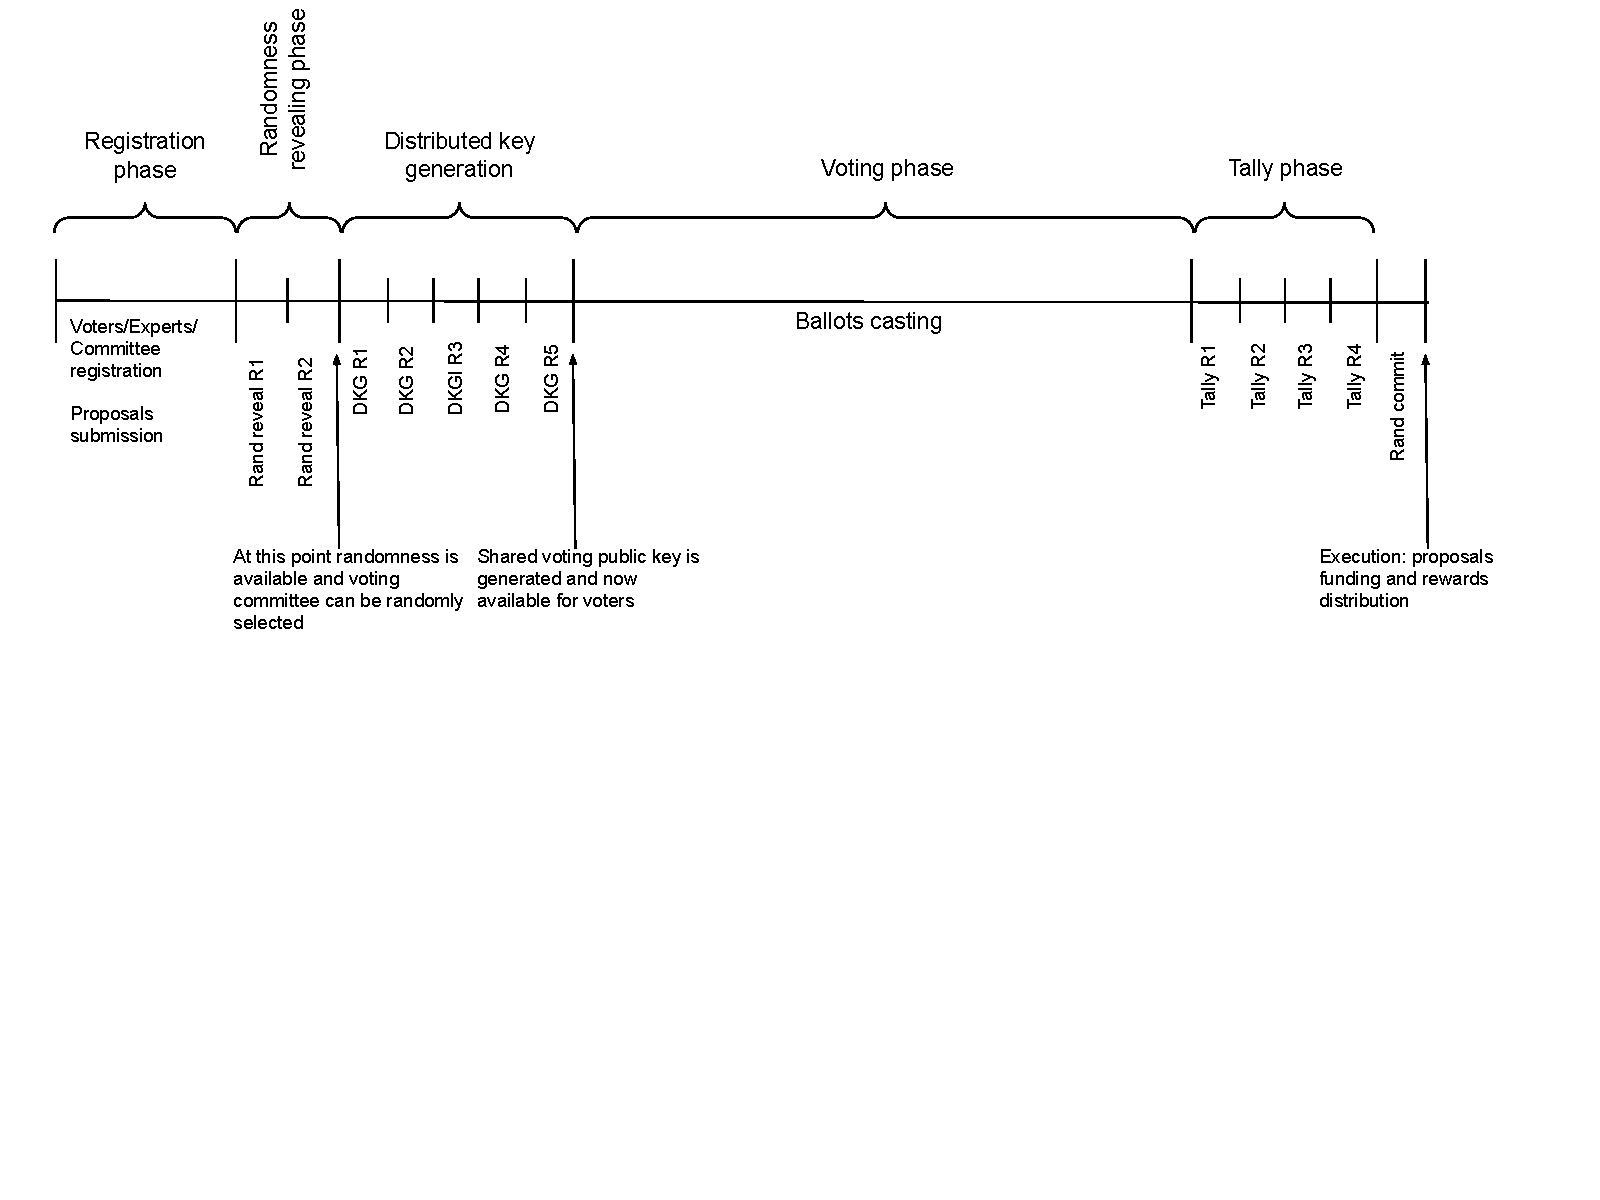
\includegraphics[trim={0.5cm 9.5cm 1.5cm 0cm}, clip,width=1\columnwidth] {treasury_epoch_timeline.pdf}
	\caption{Treasury epoch timeline}
	\label{fig:timeline}
\end{figure}